\documentclass{article}           % Sets style/look of many things.
% \documentclass{report}          % part, chapters, front page etc.
\usepackage{exsheets}
\usepackage[utf8]{inputenc}       % Encoding of input files UTF-8
\usepackage[T1]{fontenc}
\usepackage[scaled]{beramono}     % Font
\usepackage{color}                % Color text
\usepackage{titlesec}             % Select alternative section titles
\usepackage{fancyvrb}
\usepackage{verbatim}             % Comment environment
\usepackage{listings}             % Format and render text/code etc.
\usepackage{minted}               % Much better syntax highlighting
\usepackage{float}                % Control of floating environment/figure
\usepackage{graphicx,  subfigure} % Better figures, graphics, units etc.
\usepackage{multicol}             % Multiple columns
\usepackage{amsmath}              % Math: Equation, split, align etc.
\usepackage{siunitx}              % SI units
\usepackage{mathtools}            % Different math tools to use with amsmath
\usepackage{amssymb}              % Math symbols
\usepackage[
    colorlinks,
    citecolor=black,              % I like links with standard black color
    filecolor=black,
    linkcolor=black,
    urlcolor=black
]{hyperref}                       % Links in TOC etc.
\usepackage[all]{hypcap}          % Better links to floating environment

\usepackage{tabto}
\newcommand\marginsymbol[1][0pt]{%
    \tabto*{0cm}\makebox[\dimexpr-1cm-#1\relax][r]{$\mathbb{P}$}\tabto*{\TabPrevPos}}

\renewcommand{\thesubsection}{\thesection.\alph{subsection}}

% Make margins smaller to fit more figures, tables etc on page: (optional)
\addtolength{\oddsidemargin}{-1.0in}
\addtolength{\evensidemargin}{-1.0in}
\addtolength{\textwidth}{2.0in}
\addtolength{\topmargin}{-0.8in}
\addtolength{\textheight}{1.6in}

\title{\vspace{-2cm}INF3490/INF4490 Exercise Solutions - Particle Swarms \& Cartesian Genetic Programming}
\author{Eivind Samuelsen\footnote{See \href{https://github.com/olehermanse/INF3490-AI_Machine_Learning/blob/master/README.md}{\textbf{README}} for complete list of authors/contributors.}
}
\date{}

% Removing paragraph indents is sometimes useful:
\setlength\parindent{0pt}
% ==============================================================================

% ================================= DOCUMENT ===================================
\begin{document}
    \renewcommand\marginsymbol[1][0pt]{%
  \tabto*{0cm}\makebox[-1cm][c]{$\mathbb{P}$}\tabto*{\TabPrevPos}}

\maketitle
\(\mathbb{P}\) marks the programming exercises, we strongly recommend using
the python programming language for these. Exercises may be added/changed
after publishing.


\section{Particle Swarm Optimizations}
The particle swarm velocity update formula is
\begin{equation}
    v_i^{(t+1)} \leftarrow \alpha v_i ^{(t)} + U(0,\beta)(p_i-x_i^{(t)}) + U(0,\beta)(p_g - x_i^{(t)})
\end{equation}
If we replaced the random terms related to personal and global best with a term proportional to the local objective function gradient, like this:
\begin{equation}
    v_i^{(t+1)} \leftarrow \alpha v_i ^{(t)} + \gamma \nabla f(x_i^{(t)})
\end{equation}
How would the particles behave? How does this compare to gradient ascent?\\

\textit{Answer:}

The only thing separating it from doing a bunch of gradient ascent runs is the term \(av_i^{(t)}\), that transfers a fraction of the displacement in the latest iteration, giving the particles a sort of momentum.
The particles would behave as balls that roll upwards instead of downwards.

\section{Cartesian Genetic Programming}
\begin{figure}[H]
\begin{center}
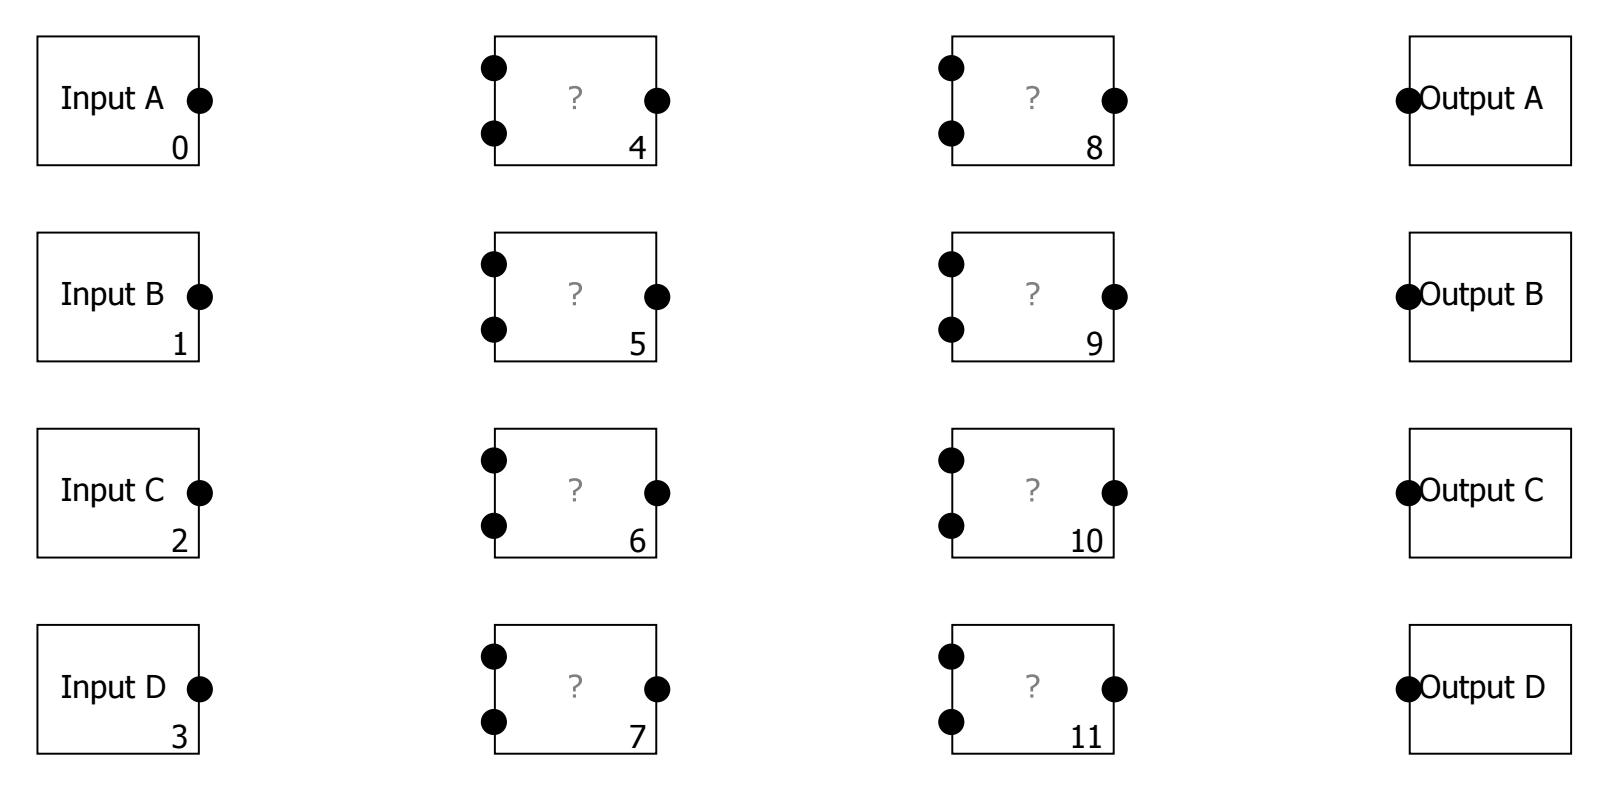
\includegraphics[width=0.9\textwidth]{cartesian.png}
\end{center}
\end{figure}
Using the setup above, construct circuits from the Cartesian genetic programming genotypes below:
\begin{itemize}
    \item 231 110 323 121 165 046 154 176 11 5 8 9
    \item 003 332 123 010 167 075 345 365 9 10 11 4
\end{itemize}

It isn't really necessary to know what the function numbers mean in order to draw the diagram.

The functions could be anything from simple binary operators (AND, OR, XOR, etc.) to real-valued arithmetic operators, to signal processing operations and so on.

\begin{figure}[H]
\begin{center}
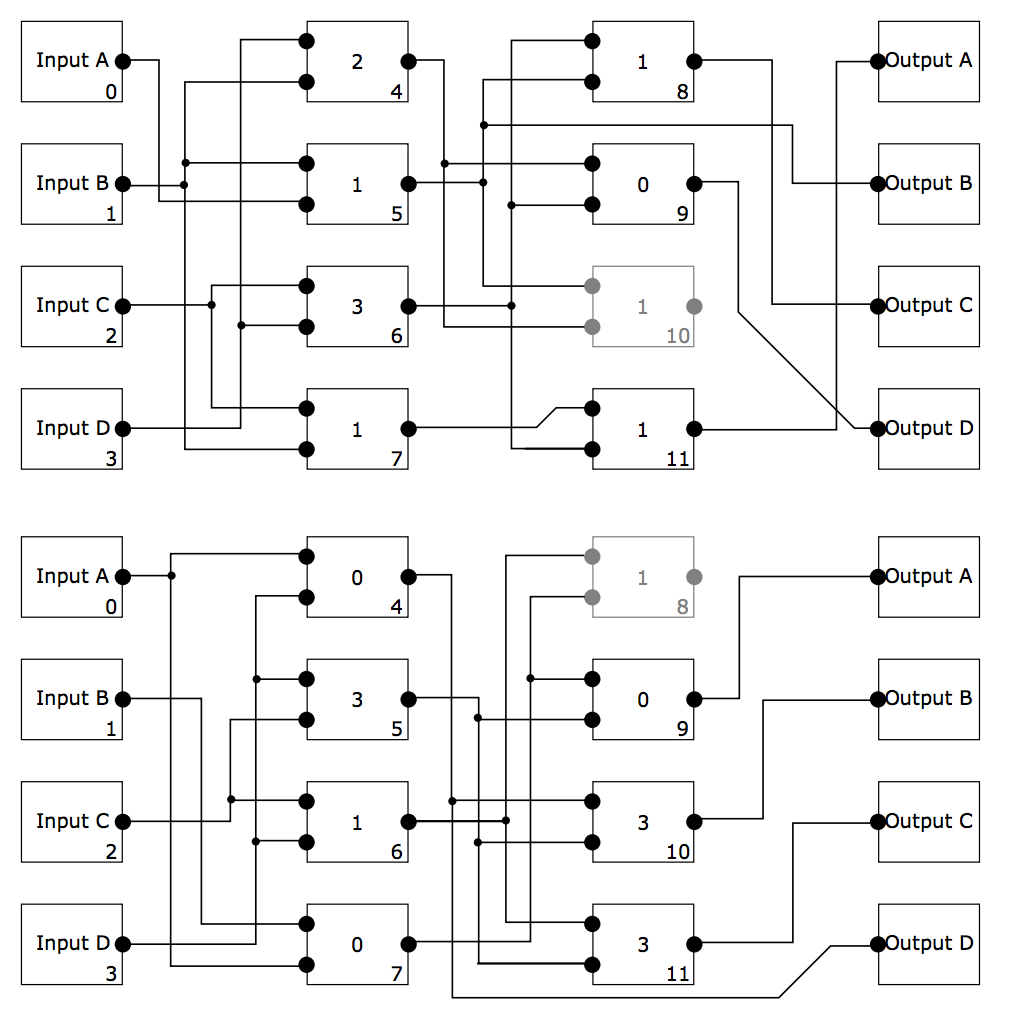
\includegraphics[width=0.6\textwidth]{cgp_sol.png}
\end{center}
\end{figure}

\section*{Contact and Github}
Corrections of grammar, language, notation or suggestions for improving this material are appreciated.
E-mail me at \href{mailto:olehelg@uio.no}{\textbf{olehelg@uio.no}} or use \href{https://github.com/olehermanse/INF3490-AI_Machine_Learning}{\textbf{GitHub}} to submit an issue or create a pull request.
The \href{https://github.com/olehermanse/INF3490-AI_Machine_Learning}{\textbf{GitHub repository}} contains all source code for assignments, exercises, solutions, examples etc.
As many people have been involved with writing and updating the course material, they are not all listed as authors here.
For a more complete list of authors and contributors see the \href{https://github.com/olehermanse/INF3490-AI_Machine_Learning/blob/master/README.md}{\textbf{README}}.

\end{document}
% ==============================================================================
